\documentclass[11pt,oneside,a4paper,titlepage,onecolumn]{article}

\usepackage[utf8]{inputenc}
\usepackage{textcomp}
\usepackage[official]{eurosym}
\usepackage[polish]{babel}
\usepackage{amsthm}
\usepackage{graphicx}
\usepackage[T1]{fontenc}
\usepackage{scrextend}
\usepackage{hyperref}
\usepackage{xcolor}
\usepackage{enumitem}
% \usepackage{nameref}
% \usepackage{showlabels}
% \usepackage{titlesec}
\usepackage{geometry}
\geometry{a4paper, portrait, margin=2cm}
\graphicspath{ {./fig/} }

\newenvironment{enumreq}
{ \begin{enumerate}[topsep=0pt,itemsep=-1ex,partopsep=1ex,parsep=1ex] }
{ \end{enumerate}                  } 


\setcounter{secnumdepth}{4}

%% Author and title
\author{Marek Marecki \and Krzysztof Franek}
\title{%
    Proving viability of Viua VM \\
    \large Implementation of high-level language on Viua VM\\
    and deployment of simple application \\
    ~\\
    Scenariusz Przypadków Użycia\\
    dla czatu ViuaChat}

\begin{document}

\maketitle
{\footnotesize
\begin{center}
  \begin{tabular}{ | l | l | l | }
    \hline
    \parbox[t]{6.5cm}{\textbf{Temat pracy i akronim projektu:}\\Proving viablity of Viua VM (VVIA)} & \parbox[t]{4.5cm}{\textbf{Zleceniodawca:}\\\colorbox{yellow}{Nieznany}} & \parbox[t]{4.5cm}{\textbf{Konsultant:}\\\colorbox{yellow}{Nieznany}} \\ \hline
    \parbox[t]{6.5cm}{\textbf{Zespół projektowy:}\\Krzysztof Franek, Marek Marecki} & \parbox[t]{4.5cm}{\textbf{Kierownik projektu:}\\Marek Marecki} & \parbox[t]{4.5cm}{\textbf{Opiekun projektu:}\\dr hab. Marek A. Bednarczyk, prof. PJWSTK} \\ \hline
    \parbox[t]{3.5cm}{\textbf{Kierownik projektu:}\\Marek Marecki} & \multicolumn{2}{|l|}{\parbox[t]{9cm}{\textbf{Odpowiedzialny za dokument:}\\Krzysztof Franek}} \\ 
    \hline
  \end{tabular}
\end{center}
}

\section{Diagramy Przypadków Użycia}

\subsection{Opis aktorów}
\textit{Należy wypełnić opis wszystkich aktorów, wchodzących w interakcje z systemem. Jeśli to uzasadnione należy dodać diagram prezentujący związki pomiędzy aktorami, np. dziedziczenie}

\begin{enumerate}
	\item \textbf{Aktor 1} – \textit{Krótka charakterystyka aktora z uwzględnieniem udziałowców, jakich reprezentuje oraz podziału: aktywny/pasywny, główny/drugorzędny}
\end{enumerate}

\subsection{Diagram Przypadków Użycia}
\begin{figure}[h]
	\centering
	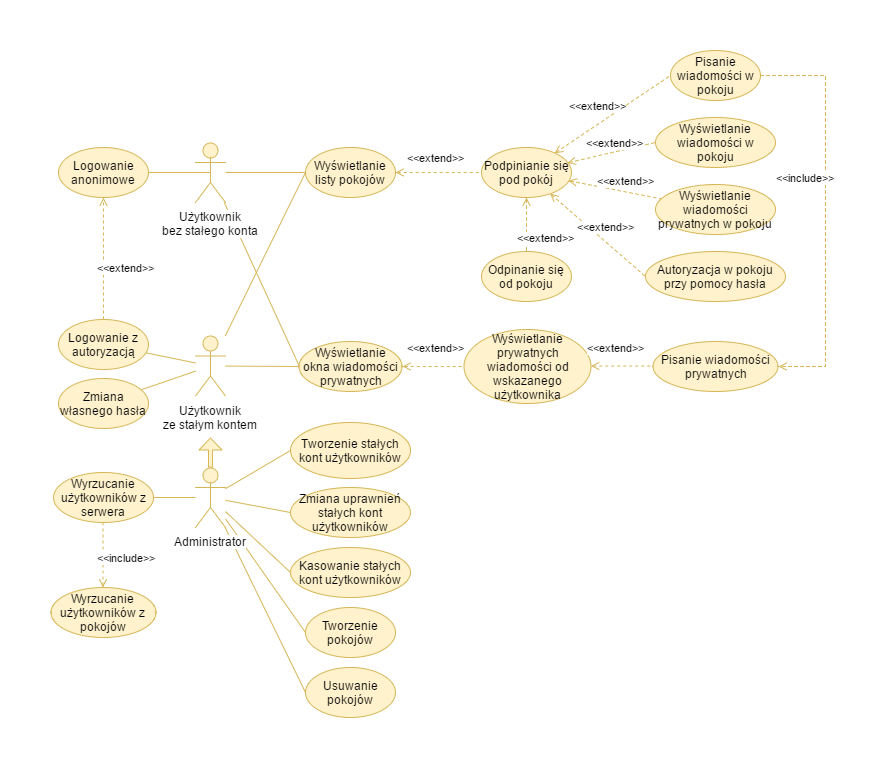
\includegraphics[width=\textwidth]{viuavm-dpu}
	\caption{Diagram przypadków użyccia}
\end{figure}

\subsection{Specyfikacja przypadków użycia}

\subsubsection{UC (nazwa przypadku)}

\begin{tabular}{ | l | l | }
	\hline
		\textbf{Identyfikator} & 
	...
		\\
		
	\hline
		\textbf{Nazwa} & \parbox[t]{13cm}{
			...
		}\\

	\hline
	
		\textbf{Aktorzy} & \parbox[t]{13cm}{
			...
		}\\

	\hline
	
		\textbf{Wymagania wstępne} & \parbox[t]{13cm}{
			...
		}\\

	\hline
	
		\textbf{Warunki wstępne i końcowe} & \parbox[t]{13cm}{
			...
		}\\
	
	\hline
	
		\textbf{Opis} & \parbox[t]{13cm}{
			...
		}\\
		
		\hline
	
		\textbf{Scenariusz podstawowy} & \parbox[t]{13cm}{
			...
		}\\
		
		\hline
	
		\textbf{Scenariusze alternatywne} & \parbox[t]{13cm}{
			...
		}\\
		
		\hline
	
		\textbf{Uwagi} & \parbox[t]{13cm}{
			...
		}\\
	
	\hline
\end{tabular}

\subsection{Diagramy sekwencji}

\subsubsection{Nazwa diagramy}


\end{document}
